\newcommand\toplisting[0]{\hrule\vspace{5px}}
\newcommand\bottomlisting[0]{\vspace{4px}\hrule}

\newcommand\customlisting[4]{
  \begin{figure}[htp]
    \centering
    \begin{minipage}{#2\linewidth}
      \toplisting
      \lstset{caption=#3,label=#1}
      \input{#4}
      \bottomlisting
    \end{minipage}
  \end{figure}
}

\newcommand\transportInterface[1]{
  \begin{figure}[htp]
    \centering
    \begin{minipage}{0.8\linewidth}
      \toplisting
      \input{scala-js-transport/transport/shared/transport/Transport.listings}
      \lstset{caption=#1,label=transportInterface}
      \input{scala-js-transport/transport/shared/transport/package.listings}
      \bottomlisting
    \end{minipage}
  \end{figure}
}

\newcommand\actorWrapper[1]{
  \customlisting{actorWrapper}{0.92}{#1}
    {scala-js-transport/examples/report-listings/src/main/scala/examples/ActorWrapper.listings}
}

\newcommand\yellingActor[1]{
  \customlisting{yellingActor}{0.68}{#1}
    {scala-js-transport/examples/report-listings/src/main/scala/examples/YellingActor.listings}
}

\newcommand\rpcExample[1]{
  \begin{figure}[htp]
    \centering
    \begin{minipage}{0.74\linewidth}
      \toplisting
      \input{scala-js-transport/examples/report-listings/src/main/scala/examples/RpcExampleApi.listings}
      \vspace{12px}
      \input{scala-js-transport/examples/report-listings/src/main/scala/examples/RpcExampleServer.listings}
      \vspace{12px}
      \lstset{caption=#1,label=rpcExample}
      \input{scala-js-transport/examples/report-listings/src/main/scala/examples/RpcExampleClient.listings}
      \bottomlisting
    \end{minipage}
  \end{figure}
}

\newcommand\engineInterface[1]{
  \customlisting{engineInterface}{0.68}{#1}{engine.listings}
}

\newcommand\stateGraph[1]{
  \begin{figure}[htp]
    \centering
    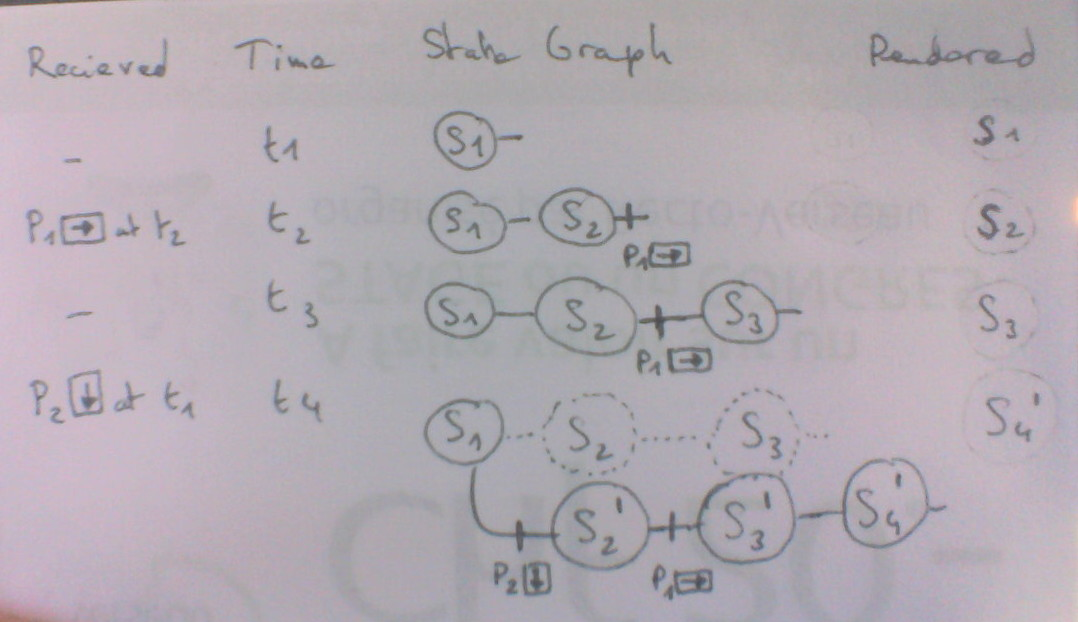
\includegraphics[width=1\textwidth]{state-graph}
    \caption{#1}
    \label{stateGraph}
  \end{figure}
}
